%KECReportFormat.tex
%%%%%%%%%%%%%%%%%%%%%%%%%%%%%%%%%%%%%%%%%%%%%%%%%%%%%%%%%%%%%%%%%%%%%%%%%%%
%DO NOT MAKE CHANGES IN THIS FILE

\documentclass[12pt, a4paper]{report}
\usepackage[left = 1.5in, right = 1in, top = 1in, bottom = 1in]{geometry}%for margin
\usepackage{amsfonts, amsmath, amssymb} %for mathematical equations
\usepackage{graphicx} %for images
\usepackage{times} %font Times New Roman Font
\usepackage{float} %required if you use H(strictly here) position for floats
\usepackage[skip = 8pt,tableposition=top, figureposition=bottom]{caption}%adjust spacing of captions and specify where captions are
\usepackage{hyperref} % for easy Navigation in document, also puts links in TOC, LOF, LOT...
\usepackage{setspace} %to change line spacing in some portion \singlespacing \onehalfspacing \doublespacing
\usepackage{acro} %for List of Abbrreviation and Symbol
\acsetup{first-style = short} % set to display only short form on the command \ac{}

%packages required for complex tables
\usepackage{bigstrut} 
\usepackage{multirow}

\renewcommand{\contentsname}{Table of Contents} %Change TOC Heading ... default is "Contents" 

\parindent 0pt	%removes the indent in paragraph
\setlength{\parskip}{18pt}	%for paragraph spacing
\renewcommand{\baselinestretch}{1.5}   %Line Spacing = 1.5 line-spaces

%to reduce spacing in sections
\usepackage{titlesec}
\titlespacing*{\section}{0pt}{0pt}{0pt} %left, top, bottom spacings
\titlespacing*{\subsection}{0pt}{0pt}{0pt}
\titlespacing*{\subsubsection}{0pt}{0pt}{0pt}
\titlespacing*{\paragraph}{0pt}{0pt}{0pt}
\titlespacing*{\subparagraph}{0pt}{0pt}{0pt}

%adjust fontsizes\ of sections
\titleformat*{\section}{\fontsize{14pt}{18pt}\bfseries}
\titleformat*{\subsection}{\fontsize{13pt}{18pt}\bfseries}
\titleformat*{\subsubsection}{\fontsize{12pt}{18pt}\bfseries}
\titleformat*{\paragraph}{\fontsize{12pt}{18pt}\bfseries}
\titleformat*{\subparagraph}{\fontsize{12pt}{18pt}\bfseries}

%to reduce separation between points in list
\usepackage{enumitem}
\setlist[enumerate]{nosep} % no separation between items in enumerate
\setlist[itemize]{nosep} % no separation between items in itemize
%use \vspace{-18pt} before list to reduce paragraph spacing between list and preceeding paragraph.

%Changes for Chapter Heading Spacing and formats for numbered chapters
\makeatletter
\def\@makechapterhead#1{%
  %\vspace*{50pt}%
  {  \MakeUppercase{\ifnum \c@secnumdepth >\m@ne
        \fontsize{16pt}{1}\bfseries \@chapapp \space \thechapter\vspace{5pt}\\
    \fi
    \interlinepenalty\@M
     \bfseries #1}\par\nobreak
    %\vskip 0pt
  }}
\makeatother

%%%%%%%%%%%%%%%%%%%%%%%%%%%%%%%%%%%%%%%%%%%%%%%%%%%%%%%%%%%
%to adjust Heading spacings and fonts For unnumbered chapters, TOC, LOF ...
\makeatletter
% Redefine the \chapter* header macro to remove vertical space
\def\@makeschapterhead#1{%
  %\vspace*{50\p@}% Remove the vertical space
  {\newpage \parindent \z@ \raggedright
    \normalfont
    \interlinepenalty\@M
    \center \fontsize{16pt}{1} \bfseries \MakeUppercase{#1}\par\nobreak
    %\vskip 18\p@ % adjust space after heading 18pt
  }}
\makeatother 
%%%%%%%%%%%%%%%%%%%%%%%%%%%%%%%%%%%%%%%%%%%%%%%%%%%%%%%%%%%

%%%%%%%%%%%%%%%%%%%%%%%%%%%%%%%%%%%%%%%%%%%%%%%%%%%%%%%%%%%%%%%%%%%%%%%%%%%
% newcommand for generating Cover Page
\newcommand{\KECcoverpage}
{
\begin{titlepage}
\begin{center}
\Large{\textbf{KANTIPUR ENGINEERING COLLEGE}}\\
\large{\textbf{(Affiliated to Tribhuvan University)}}\\
\large{\textbf{Dhapakhel, Lalitpur}}\\
\vfill	%vertically fill the space 
\begin{figure}[h] % h: put logo "here"
\begin{center}

\includegraphics[width=25mm, height = 25mm]{images/logo.png}
\end{center}
\end{figure}

\large{\textbf{[Subject Code: \subCode]}}\\ %Change This Line
\large{\textbf{A \MakeUppercase{\project} \MakeUppercase{\doc} ON}}\\ %Change This Line
\Large{\textbf{\MakeUppercase{\projectTitle}}}\\

\vfill	%vertically fill the space 
\large{\textbf{Submitted by:}}\\
\large{\textbf{\submittedBy}}\\
\vfill	%vertically fill the space 
\textbf{A \MakeUppercase{\project} SUBMITTED IN PARTIAL FULFILLMENT OF THE REQUIREMENT FOR THE DEGREE OF \MakeUppercase{\degree}}\\

\vfill	%vertically fill the space 
\large{\textbf{Submitted to:}}\\
\large{\textbf{\submittedTo}}\\
\vfill
\large{\textbf{\defMonth, \defYear}}
\pagebreak
\end{center}
\end{titlepage}
}
%%%%%%%%%%%%%%%%%%%%%%%%%%%%%%%%%%%%%%%%%%%%%%%%%%%%%%%%%%%%%%%%%%%%%%%
% newcommand for generating Cover Page
%Title Page
\newcommand{\KECtitlepage}
{
\begin{titlepage}
\begin{center}
\Large{\textbf{\MakeUppercase{\projectTitle}}}\\

\vfill	%vertically fill the space 

\large{\textbf{Submitted by:}}\\
\large{\textbf{\submittedBy}}\\

\if{\ne{\supervisor}{none}} \\ Displays Supervisor name only if it is not "none"
	\vfill	%vertically fill the space 
	\large{\textbf{Supervised by:}}\\
	\large{\textbf{\supervisor}}\\
	\large{\textbf{\degSup}}\\
\fi
\vfill	%vertically fill the space 
\textbf{A \MakeUppercase{\project} SUBMITTED IN PARTIAL FULFILLMENT OF THE REQUIREMENT FOR THE DEGREE OF \MakeUppercase{\degree}}\\

\vfill	%vertically fill the space 
\large{\textbf{Submitted to:}}\\
\large{\textbf{\submittedTo}}\\
\large{\textbf{Kantipur Engineering College}}\\
\large{\textbf{Dhapakhel, Lalitpur}}\\

\vfill
\large{\textbf{\defMonth, \defYear}}
\thispagestyle{empty}\\ %to remove page number
\pagebreak
\end{center}
\end{titlepage}
}
%%%%%%%%%%%%%%%%%%%%%%%%%%%%%%%%%%%%%%%%%%%%%%%%%%%%%%%%%%%%%%%%%%%%%%
%command for copyright page
\newcommand{\KECcopyright}
{
\chapter*{Copyright}%Required only for Final Defense of Major Project
\addcontentsline{toc}{chapter}{Copyright}
The author has agreed that the library, Kantipur Engineering Collage, may make this report freely available for inspection. Moreover the author has agreed that permission for extensive copying of this report for scholarly purpose may be granted by the supervisor(s), who supervised the project work recorded herein or, in their absence, by the Head of the Department wherein this project was done. It is understood that due recognition will be given to the author of this report and to the \submittedTo, Kantipur Engineering College in any use of the material of this report. Copying or publication or other use of this report for financial gain without approval of the \submittedTo, Kantipur Engineering College and author’s written permission is prohibited.\par Request for permission to copy or to make any other use of the material in this report in whole or in part should be addressed to:

Head\\
\submittedTo\\
Kantipur Engineering College\\
Dhapakhel, Lalitpur\\
Nepal
}
%%%%%%%%%%%%%%%%%%%%%%%%%%%%%%%%%%%%%%%%%%%%%%%%%%%%%%%%%%%%%%%%%%%%%%
%command for Approval Letter
\newcommand{\KECapproval}
{
\chapter*{Kantipur Engineering College
\vskip -10pt}%Required only for Final Defense of Major Project
\begin{center}
\fontsize{12.8pt}{1} %size decreaced to adjust department name in single line
\textbf{
\MakeUppercase{\submittedTo}\\ %for department name
}
\vskip 10pt
\fontsize{16pt}{1}
\textbf{APPROVAL LETTER}
\end{center}
\vskip -16pt
\addcontentsline{toc}{chapter}{Approval Letter}%
The undersigned certify that they have read and recommended to the Institute of Engineering for acceptance, a project report entitled "\projectTitle " submitted by \\
\submittedBy \\
in partial fulfillment for the degree of \degree. \par
{\vspace{25pt}
..........................................\\
Supervisor\\
\supervisor \\
\degSup\\
\vspace{25pt}\\
..........................................\\
External Examiner\\
\external\\
\degExternal\\
\vspace{25pt}\\
..........................................\\
\hod\\
Head of Department\\
\submittedTo
\vspace{10pt}\\
Date: \defMonth\space\defDay ,\space \defYear
\singlespacing\par
} %single spacing for the texts inside {}
}

%command for list of abbreviations
\newcommand{\KECloa}
{
\chapter*{List of Abbreviations}
\addcontentsline{toc}{chapter}{List of Abbreviations}
\vskip -42pt % to reduce space due to invisivle acronym class name
{
\singlespacing
\printacronyms[include=abbr, name= ]
}

}

%command for list of symbols
\newcommand{\KEClos}
{
\chapter*{List of Symbols}
\addcontentsline{toc}{chapter}{List of Symbols}
\vskip -42pt % to reduce space due to invisivle acronym class name{
{
\singlespacing
\printacronyms[include
=symbol, name= ]
}
}

%command to adjust toc, lof, lot spacing
\newcommand{\KECadjusttocspacings}
{
\parskip 0pt % to remove paragraph spacing in TOC, LOF ...
\renewcommand{\baselinestretch}{0.1} % to adjust line spacing in toc
\newcommand*{\noaddvspace}{\renewcommand*{\addvspace}[1]{}}
\addtocontents{lof}{\protect\noaddvspace} %remove extra vertical space in LOF
\addtocontents{lot}{\protect\noaddvspace} %remove extra vertical space in LOT
} %includes the file KecReportFormat.tex that include all necessary formattings
%%%%%%%%%%%%%%%%%%%%%%%%%%%%%%%%%%%%%%%%%%%%%%%%%%%%%%%%%%%%%%%%%%%%%%%%%%%
%Define Macros for Details of your Project
\newcommand{\project}{Major Project} %Specify "Major Project" or "Minor Project"
\newcommand{\projectTitle}{End-To-End Encryption and Decryption Using Cryptography (Asymmetric Key Encryption and Decryption (RSA)) } %specify "Title" of Your Project
\newcommand{\doc}{Proposal} % specify the document you are preparing eg. "Proposal", "Mid-Term Report" or "Final Report" 
% Note that You have to sibmit "Final Report" for Pre-final defense as well.
\newcommand{\subCode}{CT707} %specify Subject of Your Project
\newcommand{\degree}{Bachelor in Computer Engineering} %specify your degree
\newcommand{\submittedBy}%Specify Names and Roll/Symbol Numbers of the Project Group Members
{
%Edit Member Names and Roll/Symbol No. and adjust width (\makebox[width]) if necessary 
\makebox[7cm]{Anup chaudhary \hfill [KAN075BCT009]}\\
\makebox[7cm]{Chris Gurung \hfill [KAN075BCT023]}\\
\makebox[7cm]{Himalaya Pal \hfill [KAN075BCT029]}\\
\makebox[7cm]{Kundan Giri \hfill [KAN075BCT030]}
%\makebox[9cm]{Member Name \hfill [Roll/Symbol No.]}\\
} % Note that You must write your "Symbol Numbers"(Exam Roll Numbers) for Final Defenses

\newcommand{\submittedTo}{Department of Computer and Electronics Engineering} %specify your department
\newcommand{\hod}{Er. Rabindra Khati} %specify Head ot the department
\newcommand{\defYear}{2022} %Defense Year
\newcommand{\defMonth}{June} %Defense Month- January, February, ...
\newcommand{\defDay}{12} %specify Defense Day- 1, 2, ...

\newcommand{\supervisor}{none} % Specify Name of Supervisor for Major Project (write "none" if no Supervisor is assigned)
\newcommand{\degSup}{Supervisor's Designation\\Second Line of Designation (if required)} %Specify Designation of Supervisor for Major Project, use multiple lines (\\) if necessary
\newcommand{\external}{External's Name} %Specify Name of External for Major Project (Required for Black Book)
\newcommand{\degExternal}{External's Designation\\Second Line of Designation (if required)} %Specify Name of External for Major Project (Required for Black Book) , use multiple lines (\\) if necessary
%%%%%%%%%%%%%%%%%%%%%%%%%%%%%%%%%%%%%%%%%%%%%%%%%%%%%%%%%%%%%%%%%%%%%%%%%%%

%%%%%%%%%%%%%%%%%%%%%%%%%%%%%%%%%%%%%%%%%%%%%%%%%%%%%%%%%%%%%%%%%%%%%%%%%%%
%Define Abberviations and Symbols
% NOTE that Only those Abberviations and Symbols that are included in document(using command \ac{}) will be displayed in the List of Abberviations and Symbols.

%class 'abbr': for List of Abbreviations
\DeclareAcronym{HTML}{ 
  short = HTML ,
  long  = Hypertext Markup Language ,
  tag = abbr
}% declares acronym named "UN". Use \ac{UN} for short and \acl{UN} for long form. 

\DeclareAcronym{CSS}{
  short = CSS ,
  long  = Cascading Style Sheet ,
  tag = abbr
}


%%%%%%%%%%%%%%%%%%%%%%%%%%%%%%%%%%%%%%%%%%%%%%%%%%%%%%%%%%%%%%%%%
% class `symbol': for List of Symbols
\DeclareAcronym{transparencyFactor}{
  short = \ensuremath{\alpha} ,
  long  = Transparency Factor ,
  sort  = Transparency Factor , % string to compare for sorting symbols... default string is the acronym name -"transparencyFactor"
  tag = symbol
}% declares acronym named "transparencyFactor". Use \ac{UN} for short and \acl{UN} for long form.

\DeclareAcronym{areaOfTriangle}{
  short = \ensuremath{a} , % use \ensuremath{a} instead of $a$
  long  = Area of Triangle ,
  sort  = Area of Triangle , % string to compare for sorting symbols
  tag = symbol
}
%%%%%%%%%%%%%%%%%%%%%%%%%%%%%%%%%%%%%%%%%%%%%%%%%%%%%%%%%%%%%%%%%%%%%%%%%%%%%%%%%%%%%%%%%%%%%%%%%%%%

%%%%%%%%%%%%%%%%%%%%%%%%%%%%%%%%%%%%%%%%%%%%%%%%%%%%%%%%%%%%%%%%%%%%%%%%%%
%The Document
\begin{document}
\KECcoverpage % command defined in KECReportFormat
\KECtitlepage % command defined in KECReportFormat

\pagenumbering{roman} % starts pagenumberins in Roman numerals i, ii, ...

%Copyright Page is required for FINAL REPORT only. Comment this section for other Reports.
 % defined in KECReportFormat.tex

%Approval Page is required for FINAL(Black Book Binded) REPORT of MAJOR PROJECT only. Comment this section for other Reports. 
% defined in KECReportFormat.tex

\chapter*{Abstract} % The summary of your report
\addcontentsline{toc}{chapter}{Abstract}%to include this chapter in TOC 
Data security is a crucial concern that ought to be managed to help protect vital data. Cryptography is one of the
conventional approaches for securing data and is generally considered a fundamental data security component that
provides privacy, integrity, confidentiality, and authentication.

In the current world where communication has been made easy such that you could talk to a person on the other side of the world with a press of the button. With the increase in availability of internet service you can send texts, photos ,files through the internet in a matter of seconds and for far less cheaper. This is achieved through different chat applications. With the increased usage of such chat applications the contents of such messages contains more that just simple messages to friends and families but also very important information and files which on the wrong hands could cause a huge catastrophe. As such End-to-End security is needed to safely exchange private information with each other without worrying about data. With this project we aim to provide an End-to-End encrypted chat apps with file compression feature. List of requirements to make such application are provided in this paper.\cite{Chauhan2016}

This project approach End-to-end encryption method to provide  secure communication that prevents third parties from accessing data while it's transferred from one end system or device to another.
The end-to-end encryption method is implemented using the Asymmetric key encryption algorithm (RSA). We compressed the message using huffman Encoding algorithm. Then used RSA to encrypt that encoded data. The login system is also secured because we used AES library to secure the password.

In this way we can maintain the data more securely.
Since we used huffman to compress the data and RSA algorithm for securing the data.\cite{sa}

\par
\textbf{\textit{Keywords$-$}} RSA, Huffman



%to adjust spacings for TOC, LOF, LOT
{
%%%%%%%%%%%%%%%%%%%%%%%%%%%%%%%%%%%%%%%%%%%%%%%%%%%%%%%%%%%%%%%%%%%%%%%%%%%
%TOC, LOF and LOT
\KECadjusttocspacings % defined in KECReportFormat.tex to adjust spacings
\makeatletter
% to add vskip of 18 point which is reduced when parskip is set to 0 in \LECadjustspacings
\def\@makeschapterhead#1{%
	%\vspace*{50\p@}% Remove the vertical space
	{\newpage \parindent \z@ \raggedright
			\normalfont
			\interlinepenalty\@M
			\center \fontsize{16pt}{1} \bfseries \MakeUppercase{#1}\par\nobreak
			\vskip 18\p@ % adjust space after heading 18pt
		}}
\makeatother

\tableofcontents % prints table of contents
\listoffigures % prints list of figures
\addcontentsline{toc}{chapter}{List of Figures}
%\listoftables % prints list of table
%\addcontentsline{toc}{chapter}{List of Tables}
}
%%%%%%%%%%%%%%%%%%%%%%%%%%%%%%%%%%%%%%%%%%%%%%%%%%%%%%%%%%%%%%%%%%%%%%%%%%%

%comment this chapter if you don't have List of Abbreviations
%\KECloa % defined in KECReportFormat
%comment this chapter if you don't have List of Symbols
%\KECl1os % defined in KECReportFormat

\newpage
\pagenumbering{arabic} % starts pagenumbering in arabic numerals

\chapter{Introduction}
\section{Background}\label{sec:bkgrnd}%label your section if you require to refer them somewhere else in your document.
With the rapid development of mobile devices, computers and accessibility to the internet there is growing users of different chat applications. The attracting or more so important features of any social media has become the chat feature. Such chat features provide real time messaging, file sharing which may include different photos, videos, documents, etc. Chatting has been such an important aspect of the modern world that it is expected the no. of active users currently is in billions with this number expected to increase more in the coming years. Among some of the popular chat applications Whatsapp’s monthly active users(in millions) are 2000, messenger 988, snapchat 557 to name a few.\cite{Barakat2018}

The importance of such apps was never more clearly presented as when Facebook experienced outage in 2021. In what was just a 6 hour long outage the competing apps like telegram gained a record 70 million new users.
As the dependence on chat systems grow day by day the vulnerability and assaults also increases. As such  there is increasing need to implement a secure communication

Digital communication witnesses a noticeable and continuous development in
many applications in the Internet. Hence, secure communication sessions must be
provided. The security of data transmitted across a global network has turned into a
key factor on the network performance measures. So, the confidentiality and the
integrity of data are needed to prevent eavesdroppers from accessing and using
transmitted data.

One way of to secure the communication is using End-To-End encryption which use the Cryptographic algorithm. Cryptographic algorithms are divided
into symmetric and asymmetric keys. The symmetric algorithms require a single key only for the
encryption and decryption of data. Asymmetric algorithms on the other hand require both public
and private keys for the encryption and decryption of data. The scrambling of the data is done
using the public key while the private key is made known only to the receiver which is meant for
the decryption of the data.
A maiden asymmetric algorithm was proposed by Diffie-Hellman  which ensures secured
communication as well as data security. A counter algorithm termed RSA which has lower time
complexity based on prime number factorization was proposed in 1977 and is the patent of Ron
Rivest, Adi Shamir, and Len Adleman (RSA), which was published in 1978 at the Massachusetts
Institute of Technology . In this algorithm, two prime numbers are used to produce the public
and the private key. When the keys are created, the prime numbers are no more considered and
are or can be discarded.\cite{sa}

\pagebreak
\section{Problem statement}
\vspace{-18pt}
The purpose of this project is to provide the correct data with security to the users. For
some of the users the data might be lost during the transmission process in the network
and for some, the data might be changed by the unauthorized person in the network and
there are some other security problems in the network. Our application will give you more
Security to the data present in the network and there will be able to reduce the loss of data
in the network which will be transmitted from the sender to the receiver using the latest
technologies. Only the Authorized persons i.e., who are using our application will be
there in the Network.

The proposed algorithm is to compress the message at one end and ask the public key of another person and use that public key to encrypt the message and the person only decrypt the message using his private key.Using Huffman encoding the message compressed is loss less.


\section{Objectives}
The application aims to provide data security in communication system. The application focuses on
simplicity of design, having user-friendly interface and to be easily understood. \\
The main objectives of the application can be enumerated as follows:
\vspace{-18pt}
\begin{itemize}
	\item To provide end-to-end data security.
	\item To provide platform for sending messages from one person to another.
\end{itemize}

\section{Applications}
The application is an online web application. This system can be used to provide end to end encryption of data and also used to provide secure connection between user between users with smooth and clean UI.

\section{Project features}
The application, is targeted towards the general population, so the core features of this applications can be listed below:

\vspace{-18pt}
\begin{itemize}
	\item We can send messages
	\item It provides end-to-end data security in communication system.
	\item Simple and ease for general population
	\item It provides encryption, decryption and compression to messages.
\end{itemize}

\section{Feasibility Analysis}

\subsection{Economic Feasibility}
Based on our economic analysis for development and operational cost,
the system is being developed and operated economically. For development,
the required devices are readily available, so it is feasible. Also,
it is economically feasible to the consumers as it costs no charge to use the platform.

\subsection{Schedule Feasibility}
Based on the objectives and the time left for the development.
The schedule is found to be feasible.

\subsection{Technical Feasibility}
Technically, the system is feasible enough and easy-to-use
for both technical and non-technical groups of people. It provides
a user-friendly environment along with features using the latest technologies.
The system provides a layout most of the applications people are used to anyway
so it will be easy to use.

\subsection{Operational Feasibility}
For the operation of the system, the person does
not need to excel in using a computer. Since, the event
may not always be related to the technical fields, someone
with minimum knowledge about computer and technology can also get
benefit from the system. Similarly, one can get access to the system
as a web-based application. There is no requirement of huge and expensive hardware.
The system comprises only of farmer’s end.

\section{System Requirements}

\subsection{Software Requirement}
Application is targeted towards a general market,
so it is aimed to be fully optimized enough for any low-range to
high-range systems, so listed below are
the software requirements for the development and operation of this system:
\vspace{-18pt}
\begin{itemize}
	\item Operating System: Windows 8 or above
	\item Browsers: Google Chrome, Firefox, etc
	\item PostgreSQL Server
	\item Python
\end{itemize}

\subsection{Hardware Requirement}
Hardware configuration and requirements for the
operation of this application are as follows:
\vspace{-18pt}
\begin{itemize}
	\item Intel Core 2 Duo Processor (Recommended i-series processors or more) with minimum of 2GB RAM for application operation
	\item Server with optimum node speed
\end{itemize}
%\subsection{Referring Section}
%This is an example of referring Section \ref{sec:bkgrnd} of page \pageref{sec:bkgrnd}. \\



\chapter{Literature Review}
\section{Related Paper}
There are currently millions of monthly active users worldwide of different chat applications currently. There are two types of architecture in those applications, client-server and peer-to-peer networks. In a peer-to-peer network, there is no central server and each user has his/her own data storage. On the contrary, there are dedicated servers and clients in a client-server network and the data is stored on a central server. Security and privacy in chat applications have a paramount importance but few people take it seriously. In a test done by the Electronic Frontier Foundation, most of the popular messaging applications failed to meet most security standards. These applications might be using the conversations as an information for certain purposes. Moreover, reading the private conversations is certainly unacceptable in terms of privacy.  Most applications only used Transport Layer Security (TLS) for securing channel, the service provider has full access to every message exchanged through their infrastructure . Therefore, these messages can be accessed by attackers. Therefore to maintain protection and privacy, messages should be encrypted from sender to receiver and no one can read messages even the service provider, in addition to protecting the local storage of the device.\cite{paley} 

There are different Encryption algorithms that can  be utilized  to  provide secure  messaging environment. Thus, messages will circulate as  encrypted form in transmission medium, not as clear text. Somebody who has seized encrypted data does not obtain original message from the encrypted  data  unless they  possess  the  necessary  method or  a  key.  Encryption  methods  are divided into the following categories: private key cryptography and public key cryptography. 

In a symmetric key algorithm, the sender and receiver must have a shared key set up in advance and keep secret from all other parties; the sender uses this key for encryption, and the receiver uses  the  same  key  for  decryption.  In  this  case,  except  for  transmitted  encrypted  message, encryption  key  must  also  be  submitted  confidentially,  which  is  one  of  the  disadvantages of private-key cryptography.

If a third person who has managed to enter the system operator or listen to transmission medium 
seizes the  key value,  s/he can turn  the  encrypted data into  original data.  The most  important 
feature of public key cryptography which is another method is that the key value used to encrypt 
the message is different from the key value used to decrypt the message. Each user has two keys 
in this method: public key and private key. The public key of the user can be viewed by anyone. 
The private key is kept secret by the user. When someone wants to send a message to user, they 
use the user's public key and create the encrypted message and then send the encrypted data to 
user. The user  decrypts the  encrypted data with  her/his private  key  and obtains  a meaningful 
message.
 
The data which has been encrypted by the user’s public key is only solved with the user’s private key. When the user wants to send a message, s/he reaches the public key library. S/he takes 
the public key of somebody to which s/he wants to send a message and encrypts the message and 
then s/he sends the encrypted message to the receiver. The only thing that the receiver must do is 
to solve the message with his/her own private key.

RSA algorithm, which is one of the public-key encryption methods and more reliable than the 
private key encryption algorithms, is used in our proposed app for secure messaging.\cite{paley2}

RSA algorithm is asymmetric cryptography algorithm. Asymmetric means it works in two different keys: Public and Private. Public key is given to everyone and Private key is kept private.

The idea of RSA is based on the fact that it is difficult to factorize a large integer. The public key consists of two numbers where one number is multiplication of two large prime numbers. And private key is also derived from the same two prime numbers. So if somebody can factorize the large number, the private key is compromised. Therefore encryption strength totally lies on the key size and if we double or triple the key size, the strength of encryption increases exponentially. RSA keys can be typically 1024 or 2048 bits long, but experts believe that 1024 bit keys could be broken in the near future. But till now it seems to be an infeasible task.\cite{ram}

\section{Existing system:}
In this section we briefly introduce many of the popular chat applications. Some of these applications are not public or open source so it is difficult for these to get evaluated by the developer’s community, security experts or research academic.

\subsection{Viber}
Viber is an instant messaging and Voice over IP (VoIP) application for smartphones developed by Viber Media. In addition to instant messaging, users can exchange images, 
video and audio media messages. Viber recently supported the end-to-end encryption to their service, but only for one-to-one and group conversations in which all 
participants are using the latest Viber version 6.0 for Android, iOS or Windows 10. At this time, in the Viber iOS application for iPhone and iPad, attachments such as images and videos which are sent via the iOS Share Extension does not support end-to-end encryption .\cite{shyam} Viber has privacy issues such as adding a friend without his knowledge or adding him to a group without his permission. Plus that, local storage is not secured. It is not 
open source making it difficult to evaluation.

\subsection{Whatsapp}
WhatsApp is one of the most popular messaging application, recently enabled end-to-end encryption for its 1 billion users across all platforms. WhatsApp uses part of a security protocol developed by Open Whisper System, so provides a security-verification code that can share with a contact to ensure that the conversation is encrypted. It is difficult to trust in WhatsApp application completely because the application is not open source, making it difficult to verify the functioning process and match them with the work of the encryption protocol which was announced.

\subsection{Telegram}
Telegram is an open source instant messaging service enables users to send messages, photos, videos, stickers and files. Telegram provides two modes of messaging 
is regular chat and secret chat. Regular chat is client-server based on cloud-based messaging, it does not provide end-to-end encryption, stores all messages on its 
servers and synchronizes with all user devices. More, local storage is not encrypted by default. Secret chat is client-client provides end-to-end encryption. Contrary to regular chat messages, messages that are sent in a secret chat can only be accessed on the device that has been initiated a secret chat and the device that has been accepted a secret chat they cannot be accessed on other devices. Messages sent within secret chats can be deleted 
at any time and can optionally self-destruct. Telegram uses its own cryptographic protocol MTProto which is based on 256-bit symmetric AES encryption, 2048-bit RSA encryption, and Diffie–Hellman secure key exchange, and has been criticized by a significant part of the cryptographic community about its security. The registration process of Telegram, Viber and WhatsApp depend on SMS. SMS is transported via Signaling System 7 (SS7) protocol. The vulnerability lies in SS7. Attackers exploited SS7 protocol to login into 
victim's account by intercepting SMS messages. Because of Telegram cloud-based, the attacker exploits it and makes full control of the victim account and can prevent him to enter into his account. To make the account more secure should activate two-factor authentication \cite{de}

\subsection{Facebook Messenger}
Facebook Messenger is a popular messaging service 
available for Android and iOS. It provides two modes of 
messaging one is regular chat and another is secret conversations. 
Regular chat does not provide end-to-end encryption only 
secure communication by using TLS,  and it stores all 
messages on its servers. Secret conversations have  the 
same idea of Telegram secret chat . 




\chapter{Methodology}

\section{Required Algorithm:}

\subsection{Overview of  Huffman}
Huffman coding is a lossless data compression technique used widely to compress images.The main idea is to assign 
variable length codes to alphabets/symbols based upon there occurrence in the text. In this technique, the code generated is 
a prefix code, that is, if a symbol, say ‘A’, is assigned a code 0 then no other symbol can have a code starting with 0. 
It is the most efficient and widely accepted compression technique. It makes use of trees to assign codes to various 
symbols depending upon there frequency.

\subsection{Huffman Algorithm Steps:}
\vspace{-18pt}
\begin{itemize}
	\item Calculate the frequency of each symbol
	\item Take the two least frequent symbols and assign them to two leaf nodes. And assign the sum of the corresponding 
	frequencies to the parent node
	\item Now select next two least frequency nodes from the rest of the nodes along with the newly created node and form 
	another parent node,
	\item Repeat step 3 till a complete binary tree is formed
	\item  Starting from the root, assign ‘0’ to the left child and ‘1’ to the right child of every node till you reach the leaf nodes
	\item To assign the code to the symbol, trace the path from root to the corresponding node
\end{itemize}
The run time complexity of Huffman for n characters is O (n log n). 

\pagebreak
\subsection{Overview of RSA Algorithm}
RSA encryption algorithm, which is based on the idea of ensuring the secure transfer of data in the digital environment and the algorithmic difficulty of separating the integer factorization, is a type of public-key encryption method. Nowadays, it is also known as both the most commonly used encryption method and the method that allows digital signatures. It was created by Ron Rivest, Adi Shamir and Leonard Adleman  in 1978. Prime numbers are used for key generation process in RSA encryption method.This makes it possible to create a safer structure. How the encryption and decryption processes
are done with RSA algorithm is shown in below figure,
\begin{figure}[H]
	\centering
	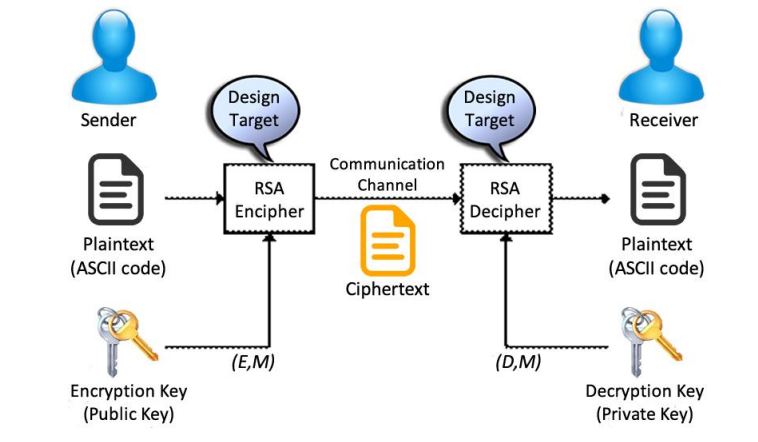
\includegraphics[width=160mm]{images/rsa algo.png}
	\caption{RSA algorithm working mechanism}
	\label{figdecisionalgo1} % for referencing
\end{figure}
\pagebreak

\subsection{RSA algorithm structure}
\subsubsection{Steps:}
\vspace{-18pt}
\begin{itemize}
	\item Choose two very large random prime integers: p and q
	\item Calculate n = p*q and z = (p-1)(q-1)
	\item Choose a number e where 1 $<$ e $<$ z
	\item Calculate d = e-1mod(p-1)(q-1)
	\item You can bundle private key pair as (n,d)
	\item You can bundle public key pair as (n,e)
\end{itemize}
After creating public and private keys, information which must be sent is encrypted with the
public key.
\subsubsection{Encryption and decryption processes are done as follows:}
\vspace{-18pt}
\begin{itemize}
	\item The cypher text C is found by the equation where M is the original
	message
	\item The message M can be found from the cypher text C by the equation M = C$^d$ mod n
	\item A text encrypted with the public key can only be solved with the private key
\end{itemize}


\pagebreak
\section{Software development model}
\subsection{Incremental Model}
\begin{figure}[H]
	\centering
	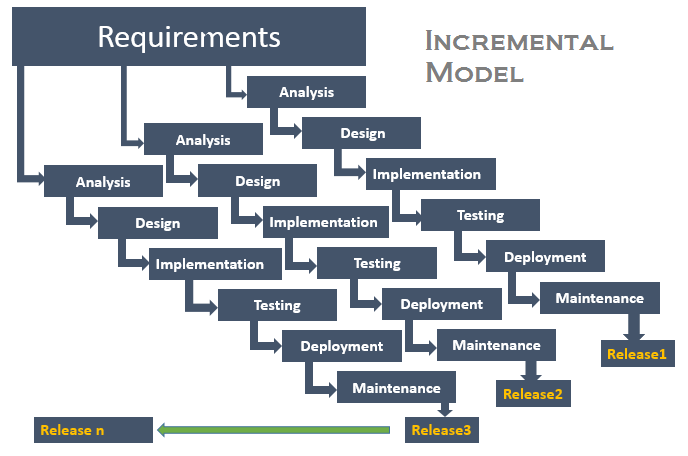
\includegraphics[width=160mm]{images/incremental model.png}{}
	\caption{Incremental Model Block Diagram} %figure name
	\label{figincremental} % for referencing
\end{figure}

\subsubsection{First Increment:}
First, the website was analyzed to know how it should look like.
Then, the designing of templates was done. After observing the design of the
templates, we started coding using react js, bootstrap, JavaScript.

\subsubsection{Second Increment:}
After analyzing the scenario of the project, the algorithms to be
implemented was analyzed. Using the algorithms, we started designing
the algorithms that is suitable for the project. Initiating the coding we
completed the algorithm implementation.
Finally, the algorithm was implemented.

\subsubsection{Third Increment:}
After the algorithm implementation backend designing and coding
was started. Using Django and Python the backend part
was completed and tested. Finally, backend was ready.

\subsubsection{Fourth Increment:}
Finally, after all the designing was completed, coding for the project was done. Later,
testing of the project was done.
At last, the final webapp was designed.
\pagebreak

\section{Block Diagram:}
\begin{figure}[H]
	\centering
	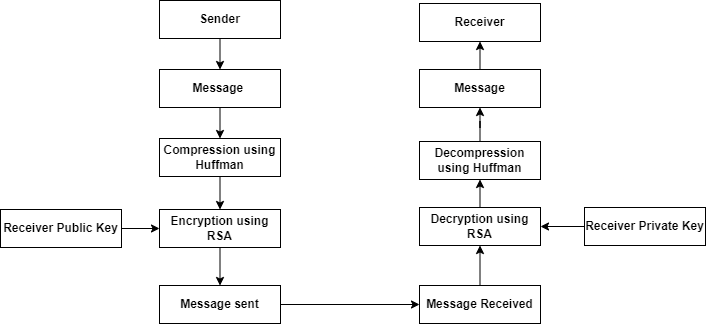
\includegraphics[width=170mm, height=160mm]{images/Block Diagram.png}
	\caption{Block Diagram} %figure name
	\label{figblockdiagram} % for referencing
\end{figure}

\section{Use Case Diagram:}
\begin{figure}[H]
	\centering
	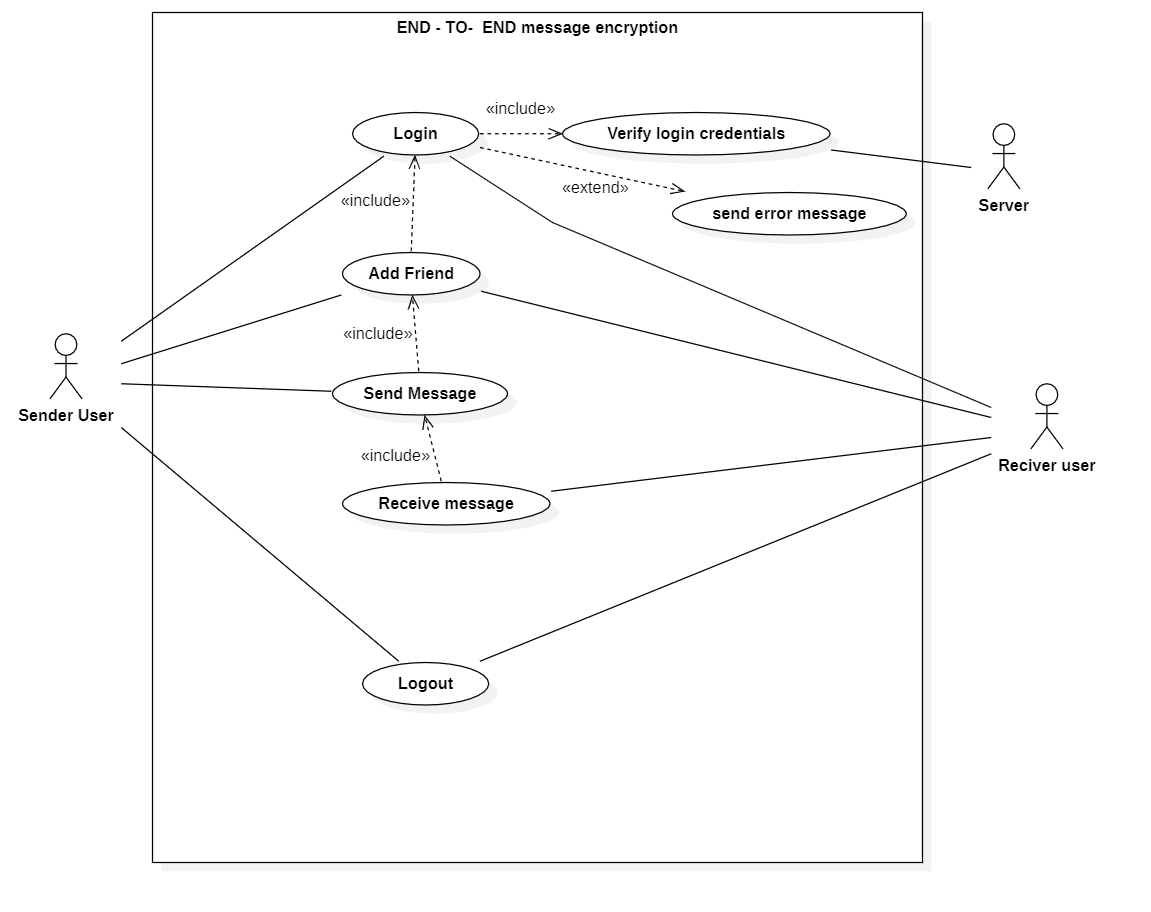
\includegraphics[width=180mm, height=180mm]{images/UseCaseDiagram1.png}
	\caption{Use Case Diagram} %figure name
	\label{figusecase} % for referencing
\end{figure}




\chapter{Epilogue}

\section{ Expected Output:}
The application will have a good user interface and user experience. It will be a web based application. In this application the user will first need  to provide their details in order to login. Then the user can send messages to receiver which is first compressed using huffman and the gets encrypted using RSA algorithm. After that same message is sent to receiver which gets decrypted using RSA algorithm and the decompressed using huffman and receiver receives message with higher security and privacy. In this the message is encrypted with public key of receiver and the decrypted using private key of receiver. We expect a clean UI of this message communication web application with higher security and privacy. 

\section{Work Schedule}
Scheduling establishes the timelines, delivery and availability of project resources whether they be personnel, inventory or capital. For this reason, any project without a schedule is a project doomed to issue down the road.

\begin{figure}[H]
	\centering
	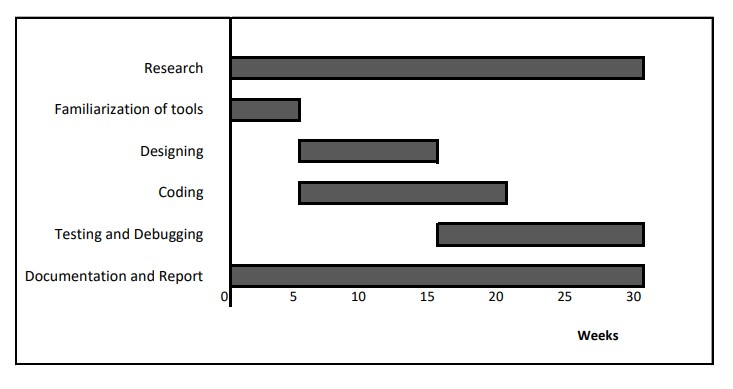
\includegraphics[width=160mm]{images/ganttchart.png}
	\caption{Gantt Chart} %figure name
	\label{figganttchart} % for referencing
\end{figure}




%Reference
\renewcommand\bibname{References} % Change heading to References
\bibliographystyle{IEEEtran} % to use IEEE Format for referencing
\addcontentsline{toc}{chapter}{References} % to add references in TOC
\bibliography{library} % specify the .bib file containing reference information 

%Comment this Chapter if you do not need to include Appendix.
%\chapter*{Appendix}
%\addcontentsline{toc}{chapter}{Appendix}
%Appendix Text Comes Here

\end{document}
